\chapter{Preliminaries}
\textit{This chapter refers to (and summarizes) my Master 1 project. Concepts and definitions are essentially inspired by the chapter 10 of the book ``Principles of model checking'' \cite{PMC}, the chapter ``Model checking probabilistic systems'' of the Mickael Randour course called ``Formal verification of computer systems'' \cite{MRV} as well as the article ``Variations on the shortest path problem'' \cite{DBLP:journals/corr/RandourRS14a}.} \\

Before studying different multi-objective problems in \textit{Markov decision
processes} and defining \textit{strategies} that solve such problems, we will introduce some fundamental concepts that define the area of the subject.
Actually, we will be interested to know some measurements related to the cost of \textit{paths} of Markov decision process as well as to the probability to reach some states in this model through these paths.
These measurements can not be computed without defining a probability measure on these paths.
So, first of all, we need to define what are \textit{Markov chains}. Indeed, these
stochastic models are essential to measure the probability of \textit{paths} of Markov decision processes.

\section{Markov chains}
\begin{definition}[\textbf{Discrete-time Markov chain}]
  A \textit{(weighted) discrete-time Markov chain} (denoted by \textbf{MC}) is a stochastic model defined by a tuple $\mathcal{M}=(S, \Delta, w, AP, L)$ where
	\begin{itemize}
		\item $S$ is a countable set of states,
		\item $\Delta: S \times S \rightarrow [0,1] \cap \mathbb{Q}$ is a  \textit{transition function} such that \[\forall s \in S, \sum_{s' \in S}\Delta(s, s')= 1\]
		%\item $d_0:S \rightarrow [0,1]$ est la distribution initiale telle que \[\sum_{s \in S}d_0(s)= 1\] (à noter que dans le cadre de ce document, la distribution initiale peut être omise, et dans ce cas, $\forall s \in S, d_0(s) = \frac{1}{|S|}$).
		where $\Delta(s, s')$ describes the probability that the system goes from state $s$ to state $s'$ in one transition,
    \item $w : S \times S \rightarrow \mathbb{N}_0$ %est la fonction
        %de poids associant à chaque transition un coût strictement positif.
      is a weight function that links a strictly positive cost to each transition,
    \item $AP$ is a set of atomic propositions, and
    \item $L : S \rightarrow 2^{AP}$ is a labeling function.
	\end{itemize}
  \textit{Note }: $AP$ and $L$ can be ommited. In that case, we will consider that $AP = S$ and $L$ is the natural labeling of each state, i.e., for all $s \in S$, $L(s) = \{s\}$
\end{definition}

\begin{property}
  Let $\mathcal{M} = (S, \Delta, w, AP, L)$ be a MC and $s \in S$ be a state of $\mathcal{M}$. The transition function $\Delta$ defines a probability distribution $\Delta_s : S \rightarrow [0, 1], \, s' \mapsto \Delta(s, s')$ on $S$.
\end{property}

We can represent a MC $\mathcal{M} = (S, \Delta, w, AP, L)$ with a directed graph, where vertices represent the states
of the MC and where all edge $(s, s') \in S^2$ that links two states is labeled with the transition probability to go from $s$ to $s'$, i.e., $\Delta(s, s')$, as well as the cost of this transition, i.e., $w(s, s')$. Additionally, the labels of each
states can be represented next to it.

\begin{example}[\textit{Production of solar pannels according to weather}]\label{solar-pannel}
  Let $\mathcal{M}_{sp} = (S, \Delta, w, AP, L)$ be the MC of the figure \ref{MCexample}. This system modelises the production of eneregy (in $kJ$) of
  an installation of solar pannels according to weather.
  Here, the states are elements of $S = \{s_0, s_1, s_2, s_3\}$ and the atomic propositions are elements of $AP = \{sunny, \, slightly\_cloudy, \, moderately\_cloudy, \, cloudy \}$. The transition function is given by edges on the figure (e.g., $\Delta(s_0, s_1) = \frac{1}{5}$) as well as the
  cost of each transition (e.g., $w(s_0, s_1) = 5$). Finaly, labels of states
  are put next each of them in orange in the figure (e.g., $L(s_0) = \{sunny\}$).
  \begin{figure}[h!]
    \centering
    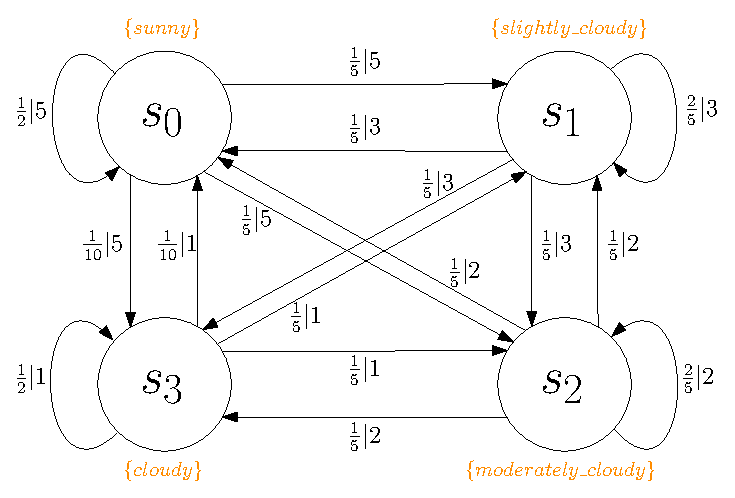
\includegraphics[width=0.6\linewidth]{resources/weather-solar-pannel}
    \caption{MC modeling a daily production of energy (in $kJ$) of solar pannels according to weather}
    \label{MCexample}
  \end{figure}
  The way $w$ is defined for this MC yields that when a day is sunny, the installation produces $5 kJ$ during this day, $3 kJ$ when a day is slightly cloudy, $2 kJ$ when a day is moderately cloudy and finaly $1 kJ$ when the day is cloudy.
\end{example}

\subsection{Probability of paths in a MC}

\begin{definition}[\textbf{Paths of a MC}] Let $\mathcal{M} = (S, \Delta, w, AP, L)$ be a MC.
A \textit{path} $\pi = s_0 s_1 s_2 \dots$ of $\mathcal{M}$ is a (infinite) sequence of states of the MC such that for all $i \in \mathbb{N}$, $\Delta(s_i, s_{i+1})> 0$. We denote by $Paths(s)$ the set of paths $\pi = s_0s_1s_2\dots$ of $\mathcal{M}$ that begin in the state $s \in S$, i.e., such that $s_0 = s$.
\end{definition}
\begin{definition}[\textbf{Finite paths of a MC}]
Let $\mathcal{M} = (S, \Delta, w, AP, L)$ be a MC.
A \textbf{finite} path $\hat{\pi} = s_0 \dots s_n$ of $\mathcal{M}$, with $n \in \mathbb{N}$, is a finite sequence of states of $\mathcal{M}$ such that $\Delta(s_i, s_{i+1}) > 0$ for all $i \in \{0, \dots, n-1\}$.
We denote by $Paths_{fin}(s)$ the set of finite paths $\hat{\pi} = s_0 \dots s_n$ that begin in the state $s \in S$, i.e., such that $s_0 = s$
\end{definition}
\begin{definition}[\textbf{Prefixes of paths}]
Let $\mathcal{M} = (S, \Delta, w, AP, L)$ be a MC and $\pi = s_0s_1s_2 \dots$ be a path of $\mathcal{M}$. A prefix of $\pi$ is a finite path $\hat{\pi} = s'_0 \dots s'_n$, with $n \in \mathbb{N}$ such that $s'_i = s_i$ for all $i \in \{0, \dots, n\}$. The set of all prefixes of $\pi$ is denoted by $pref(\pi)$
\end{definition}

We are now interested of measuring the probability of events of MCs. These events can be formulated with the notion of \textit{cylinder set}.

\begin{definition}[\textbf{Cylinder set}]
Let $\mathcal{M} = (S, \Delta, w, AP, L)$ be a MC, $s \in S$ be a state of $\mathcal{M}$ and $\hat{\pi} \in Paths_{fin}(s)$ be a finite path of $\mathcal{M}$.
\[Cyl(\hat{\pi})=\{\pi\in Paths(s)\;|\;\hat{\pi}\in pref(\pi) \} \]
\end{definition}

We can express all events with this formulation. For example, the event that consists of a singleton containing just a single path $\pi = s_0s_1\dots$ of a MC $\mathcal{M}$, is given by $\bigcap_{\hat{\pi} \in pref(\pi)} Cyl(\hat{\pi})$

\begin{theorem}\label{theo1}
  Let $\mathcal{M}=(S, \Delta, w, AP, L)$ be a MC and $s \in S$ be a state of $\mathcal{M}$. There exists a unique probability measure $\mathbb{P}_s$ on the
  $\sigma$-algebra over $Paths(s)$ where the probabilities of cylinder sets (i.e., of events) are given by
  \[
    \mathbb{P}_s(Cyl(s_0 \dots s_n)) = \prod_{i = 0}^{n - 1} \Delta(s_i, s_{i+1})
  \]
  where $s_0 = s$ and $n \in \mathbb{N}$.
\end{theorem}
\begin{corollary}
Any event defined using complementation or countable union of cylinder sets are also measurable.
\end{corollary}

\begin{example}[\textit{Probability of paths in a MC modeling a solar pannel}]
  Let $\mathcal{M}_{sp} = (S, \Delta, w, AP, L)$ be the MC of the example \ref{solar-pannel}. The probability of sunny weather four days in a row starting on a sunny day is given
  by $\mathbb{P}_{s_0}(Cyl(s_0s_0s_0s_0)) = (\frac{1}{2})^3 = \frac{1}{8}$
\end{example}

\subsection{Objectives in Markov chains}

With this background, we can now introduce some classical problems that consist
of completing an objective in a MC. The first one that we will tackle is the reachability problem.
%\subsubsection{Reachability problem}
\begin{definition}[\textbf{Reachability event}]
  Let $\mathcal{M} = (S, \Delta, w, AP, L)$ be a MC and $T \subseteq S$ be a set of target states. The event of reaching $T$, denoted by $\Diamond T$,
  is defined as a finite union of cylinder sets. Indeed, let $s \in S$ be a state of $\mathcal{M}$ and $Paths_{fin}^T(s)$ be the set of finite paths $\hat{\pi} = s_0 \dots s_n \in Paths_{fin}(s)$, $n \in \mathbb{N}$, such that $\forall i \in \{0, \dots, n-1 \}, \, s_i \not \in T$ and $s_n \in T$,
  \[ \Diamond T = \bigcup_{s_0 \dots s_n \in Paths_{fin}^T(s)} Cyl(s_0 \dots s_n) \]
  As all cylinders of the set $Paths_{fin}^T(s)$ are disjoint (their prefixes are different), we can measure the probability of $\Diamond T$ with :
  \[
    \mathbb{P}_s(\Diamond T) = \sum_{s_0 \dots s_n \in Paths_{fin}^T(s)} %Cyl(s_0 \dots s_n)
    \prod_{i=0}^{n-1} \Delta(s_i, s_{i+1})
  \]
\end{definition}
It remains to compute this probability.

\begin{theorem}
Computing $\mathbb{P}_s(\Diamond T)$ for all $s \in S$ can be done in polynomial
time through a linear equations system (cf. appendix for more details).
\end{theorem}

Now, we will consider the \textit{cost of paths} of a MC. Furthermore, we
are interrested by the cost of paths to reach $T$. To compute this cost, we use the \textit{truncated sum function}.

\begin{definition}[\textbf{Truncated sum}]
  Let $\mathcal{M}=(S, \Delta, w, AP, L)$ be a MC, $s \in S$ be a state of $\mathcal{M}$, $\pi = s_0s_1s_2\dots \in Paths(s)$ be a path of $\mathcal{M}$ and $T \subseteq S$ be a set of target states.
  The trunacted sum of $\pi$ is the cost to reach $T$ through $\pi$
  for the first time. More formally, the function $TS^T : Paths(s) \rightarrow \mathbb{N} \cup \{\infty\}$ is defined as follow :
	\[
		TS^T(\pi) =
		\begin{cases}
			\sum_{i = 0}^{n-1} w(s_i, s_{i+1}) & \quad \text{si } \forall i \in \{0, \dots, n - 1\}, s_i \not\in T \text{ et } s_n \in T \\
			\infty & \quad \text{si } \pi \not \models \Diamond T,\; \text{, i.e., } \; \forall i \;\; s_i \notin T
		\end{cases}
	\]
\end{definition}
With this function, it is now possible to introduce the concept of the
expected cost of paths of a MC to reach a set of targets as well as
the probability of reaching this target set with a cost bounded.

\begin{definition}[\textbf{Expected cost of paths of a MC for reachablity properties}]
	Let $\mathcal{M} = (S, \Delta, w, AP, L)$, a MC, $s \in S$, a state of $\mathcal{M}$ and $T \subseteq S$, a set of targets. We define the expected cost to reach $T$, i.e., $\mathbb{E}_s(\Diamond T)$, corresponding to \textit{the expected truncated sum of paths from $s$ to reach $T$} as follow :
	\begin{itemize}
	\renewcommand{\labelitemi}{\tiny$\bullet$}
	\item If $\mathbb{P}_s(\Diamond T) < 1$, then $\mathbb{E}_s(\Diamond T) = \infty$.%(par la propriété \ref{prop-ts}).
	\item Else, if $\mathbb{P}_s(\Diamond T) = 1$, then :
	\[
    \mathbb{E}_s(\Diamond T) = \sum_{c = 0}^\infty c \cdot \mathbb{P}_s(\{\pi \in Paths(s) \; | \; TS^T(\pi) = c \})
  \]
	\end{itemize}
\end{definition}

An equivalent characterisation of the expected cost from $s \in S$ to $T$ in case of $\mathbb{P}_s(\Diamond T) = 1$ is given by
\[
  \mathbb{E}_s(\Diamond T) = \sum_{\hat{\pi} \in Paths_{fin}^T(s)} \mathbb{P}_s(Cyl(\hat{\pi})) \cdot TS^T(\hat{\pi})
\]
with $Paths^T_{fin}(s)$, the set of finite paths $\hat{\pi} = s_0 \dots s_n \in Paths_{fin}(s)$  such that for all $i \in \{0, \dots, n-1\}, s_i \not \in T$ and $s_n \in T$. As we can measure the probability of cylinder sets of finite paths of $\hat{\pi} \in Paths_{fin}^T(s)$, we can compute $\mathbb{E}_s(\Diamond T)$.

\begin{theorem}
  Computing $\mathbb{E}_s(\Diamond T)$ for all $s \in S$ can be done in polynomial time through a linear equations system (cf. appendix for more details).
\end{theorem}
